% Quick start guide
\documentclass[envcountsect]{beamer}

\usepackage[utf8]{inputenc}
\usepackage[T2A]{fontenc}
\usepackage[english,russian]{babel}
\usepackage{graphicx}
\usepackage{amsmath}
\usepackage{float}
\usepackage{hyperref}
\usepackage{amssymb}
\usepackage{bbm}
\usepackage{amsthm}
\usepackage{indentfirst}
\usepackage{comment}
\usepackage[thinc]{esdiff}

\selectlanguage{russian}
\usetheme{Warsaw}

\newtheorem{rutheorem}{Теорема}
\newtheorem{rustatement}{Утверждение}
\newtheorem*{ruremark}{Замечание}
\newtheorem*{ruexample}{Пример}
\theoremstyle{definition}
\newtheorem{rudefinition}{Определение}[section]

% Title page details
\title[Условия квазимонотонности для кусочно-аффинных систем дифференциальных уравнений]{Условия квазимонотонности для кусочно-аффинных систем дифференциальных уравнений} 
\author[Миловидов М.\,В.]{Миловидов Михаил Владимирович\\ Научный руководитель --- к.ф.-м.н., доцент П.\,А.~Точилин}
\institute{Факультет ВМК МГУ имени М. В. Ломоносова, кафедра системного анализа}
\date{2 июня 2026 г.}

\setbeamertemplate{footline}{%
	\leavevmode%
	\hbox{%
		% Блок с автором (занимает 50% ширины)
		\begin{beamercolorbox}[wd=.18\paperwidth,ht=2.25ex,dp=1ex,center]{author in head/foot}%
			\usebeamerfont{author in head/foot}\insertshortauthor
		\end{beamercolorbox}%
		% Блок с датой и номером (занимает 50% ширины)
		\begin{beamercolorbox}[wd=.82\paperwidth,ht=2.25ex,dp=1ex,center]{date in head/foot}%
			\usebeamerfont{date in head/foot}\insertshorttitle
		\end{beamercolorbox}%
	}%
	\vskip0pt%
}

\begin{document}
	
	\begin{frame}
		% Print the title page as the first slide
		\titlepage
	\end{frame}
	
	\begin{frame}
		\begin{rudefinition} 
			Система
			\begin{equation} \label{sys}
				\dot x = f(x),\, x \in \mathbb{R}^n,\, n \ge 2 
			\end{equation}
			называется квазимонотонной, если
			\[\forall i \in \overline{1,n},\ \forall \alpha_j \ge 0,\ j = \overline{1,n},\ j \ne i\]
			\begin{equation} \label{qm}
				\begin{split}
				f_i(x_1+\alpha_1,\dots,x_{i-1} + \alpha_{i-1},x_i,x_{i+1}+\alpha_{i+1},\dots,x_n+\alpha_n) \ge \\  \ge f_i(x_1,\dots,x_n).
				\end{split}
			\end{equation}
			Это свойство также называется монотонностью по внедиагональным элементам, или же условием Важевского.
		\end{rudefinition}
	\end{frame}
	
\begin{comment}
	
	\begin{frame}
		Рассмотрим систему
		\begin{equation} \label{usys}
			\begin{cases} 
				\dot x = f(t, x, u),\ t \in [t_0,t_1],\\
				x(t_0) = x_0 \in \mathcal{X}_0,\\
			\end{cases}
		\end{equation}
		где \(\mathcal{X}_0 \subset \mathbb{R}^n\) --- множество начальных значений, \(u = u(t) \in \mathcal{U}\ \forall t \in [t_0,t_1]\), \(\mathcal{U} \subset \mathbb{R}^m\) --- множество допустимых управлений. Решение системы с начальным значением \(x_0 \in \mathcal{X}_0\) в момент времени \(t_0\) и допустимым управлением \(u \in \mathcal{U}\) обозначается
		\[
		x(t; t_0, x_0, u),\ t \in [t_0,t_1].
		\]
	\end{frame}
	
	\begin{frame}
		\begin{rudefinition} 
			Система
			\begin{equation}
				\dot x = f(t, x, u),\, x \in \mathbb{R}^n,\, n \ge 2 
			\end{equation}
			называется квазимонотонной, если
			\[\forall i \in \overline{1,n},\ \forall \alpha_j \ge 0,\ j = \overline{1,n},\ j \ne i,\ \forall \beta_k \ge 0,\ k = \overline{1, m}\]
			\begin{multline}	\label{uqm}
				f_i(t, x_1+\alpha_1,\dots,x_{i-1} + \alpha_{i-1},x_i,x_{i+1}+\alpha_{i+1},\dots,x_n+\alpha_n, \\ u_1 + \beta_1,\dots,u_m + \beta_m) \ge f_i(t, x_1,\dots,x_n, u_1,\dots, u_m)\ \forall t \in [t_0,t_1].
			\end{multline}
		\end{rudefinition}

	\end{frame}
	
	\begin{frame}
		\begin{rudefinition}
			Множество
			\begin{multline*}\mathcal{R}(t) = \mathcal{R}(t; t_0, \mathcal{X}_0, \mathcal{U}) = \\ = \{x \in \mathbb{R}^n: \exists x_0 \in \mathcal{X}_0,\ u \in \mathcal{U}: x = x(t; t_0, x_0, u)\},\ t \in [t_0,t_1]\end{multline*}
			называется множеством достижимости системы в момент времени \(t\).
		\end{rudefinition}
		
		\begin{rudefinition} \label{hr}
			Множество
			\[
			[\underline{x}, \overline{x}] = \{x \in \mathbb{R}^n: \underline{x}_i \le x_i \le \overline{x}_i\ \forall i = \overline{1, n}\},\ \underline{x}, \overline{x} \in \mathbb{R}^n
			\]
			называется гиперотрезком или гиперпрямоугольником.
		\end{rudefinition}
	\end{frame}
	
	\begin{frame}
		Для квазимонотонных систем верно следующее утверждение:
		\begin{rustatement}
			Пусть в системе (\ref{usys}) функция \(f\) непрерывно дифференцируема и для всех \(t \in [t_0,t_1],\ x \in \mathcal{X}_0,\ u \in \mathcal{U},\ i, j = \overline{1, n},\ i \neq j,\ k = \overline{1, m}\) выполнено
			\begin{equation} \label{jakobian}
				\diffp{f_i}{{x_j}}(t, x, u) \ge 0,\ \diffp{f_i}{{u_k}}(t, x, u) \ge 0.
			\end{equation}
			Пусть также \(\mathcal{X}_0 \in [\underline{x}, \overline{x}],\ \mathcal{U} \subset [\underline{u},\overline{u}]\). Тогда
			\[
			\mathcal{R}(t; t_0, \mathcal{X}_0, \mathcal{U}) \subset [x(t; t_0, \underline{x}, \underline{u}), x(t; t_0, \overline{x}, \overline{u})].
			\]
		\end{rustatement}
	\end{frame}
	
\end{comment}
	
	\begin{frame}
		Также введем понятие кусочно-аффинной функции.
		\begin{rudefinition}
			Функция \(f(x), x \in \mathbb{R}^n\) называется кусочно-аффинной, если она имеет вид
			\begin{equation} \label{pwadef}
				f(x) = A^{(k)}x + b^{(k)},\quad x \in \Omega^{(k)},
			\end{equation}
			где
			\[\Omega \subset \mathbb{R}^n, \Omega = \bigsqcup_{k = 1}^m \Omega^{(k)},\, x \in \mathbb{R}^{n},\, A=[a_{ij}] \in \mathbb{R}^{n \times n},\, b \in \mathbb{R}^{n}.\]
			\[f_i^{(k)}(x) = \sum_{j=1}^{n} a_{ij}^{(k)}x_j + b_i^{(k)}.\]
		\end{rudefinition}
	\end{frame}

	\begin{frame}{Постановка задачи}
		В данной работе мы будем исследовать условие квазимонотонности для частных видов кусочно-афинных (кусочно-линейных) функций. В результате нужно получить некоторые необходимые и достаточные условия. Рассмотрим следующие виды функции \(f(x)\):
		\begin{enumerate}
			\item \(\forall i = \overline{1,n}\ \, f_i(x) \) --- суперпозиция функций \(\min()\), \(\max()\) и арифметических операций.
			\item Функция \(f(x)\) определена на множестве \(\Omega \subset \mathbb{R}^n\), причем \(\Omega = \bigsqcup_{k = 1}^m \Omega^{(k)}\), где \(\Omega^{(k)}\) --- выпуклые многогранники, и функция \(f(x)\) на \(\Omega^{(k)}\) имеет вид \(f_i(x) = \sum_{j = 1}^{n} a_{ij}^{(k)}x_j + b_i^{(k)}\). Значения функции на границах обговариваются отдельно.
		\end{enumerate}
	\end{frame}
	
	\begin{frame}{Афинные системы}
		Рассмотрим афинную функцию вида
		\[f(x) = Ax + b,\, x \in \mathbb{R}^{n},\, A=[a_{ij}] \in \mathbb{R}^{n \times n},\, b \in \mathbb{R}^{n}.\]
		\[f_i(x) = \sum_{j=1}^{n} a_{ij}x_j + b_i.\]
		
		Для таких функций справедлив следующий критерий квазимонотонности:
		\begin{equation} \label{qmaff}
			a_{ij} \ge 0\ \forall i \neq j,\ i,j = \overline{1, n}.
		\end{equation}
	\end{frame}
	
	\begin{frame}{Кусочно-афинные системы}
		Пусть 
		\[f(x) = \begin{cases}A^{(k)}x + b^{(k)},\quad x \in \Omega^{(k)},\end{cases}\]
		где
		\[\Omega \subset \mathbb{R}^n, \Omega = \bigsqcup_{k = 1}^m \Omega^{(k)},\, x \in \mathbb{R}^{n},\, A=[a_{ij}] \in \mathbb{R}^{n \times n},\, b \in \mathbb{R}^{n}.\]
		\[f_i^{(k)}(x) = \sum_{j=1}^{n} a_{ij}^{(k)}x_j + b_i^{(k)}.\]
		Аналогично предыдущему случаю, получаем условие:
		\begin{equation} \label{qmpwaff}
			a_{ij}^{(k)} \ge 0\ \forall i \neq j,\ i,j = \overline{1, n},\ k = \overline{1, m}.
		\end{equation}
		Однако оно уже не будет достаточным для квазимонотонности функции. Нужно также проверять неубывание при прохождении границ множеств.
	\end{frame}
	
	\begin{frame}{Системы, являющиеся суперпозицией функций \(\min\) и \(\max\)}
		Рассмотрим суперпозицию функций \(\min\) и \(\max\), а именно функции, у которых \(f_i\) являются суперпозициями функций \(\min\), \(\max\) а также арифметических операций \(+\) и \(-\) и операции умножения на константу.
		\begin{ruexample}
			\[\begin{cases}
				f_1(x) = 1 + \min(2x_1,x_2) + \min(x_1, 2x_2), \\
				f_2(x) = -\max(2x_1 - x_2, x_2, \min(3, x_1)).
			\end{cases}\]
			\[
			f_2(x) = \begin{cases}
				-2x_1 + x_2,\ x_1 \ge x_2,\\
				-x_2,\ x_1 < x_2. \\
			\end{cases}
			\]
			Функция \(f\) не является квазимонотонной.
		\end{ruexample}
		Такие функции будут являться непрерывными, а значит, условие \ref{qmpwaff} будет также и достаточным. 
	\end{frame}
	
	\begin{frame}{Случай простой суперпозиции}
		Рассмотрим случай простой суперпозиции:
		\[f_i(x) = \max(g_i^{(1)}(x),\dots,g_i^{(m_i)}(x))\]
		или
		\[f_i(x) = \min(g_i^{(1)}(x),\dots,g_i^{(m_i)}(x)),\]
		где
		\[g_i^{(k)}(x) = \sum_{j=1}^n a_{ij}^{(k)} x_j + b_i^{(k)},\, i = \overline{1, n},\, k = \overline{1, m_i}.\]
		Для таких функций условие (\ref{qmpwaff}) принимает вид
		\begin{equation} \label{qmmm}
			a_{ij}^{(k)} \ge 0\ \forall i \neq j,\ i,j = \overline{1, n},\ k = \overline{1, m_i}.
		\end{equation}
	\end{frame}

\begin{comment}
	
	\begin{frame}{Общий случай}
		К этому случаю можно свести некоторые более сложные виды функций, однако в общем случае не всегда можно утверждать об отсутствии квазимонотонности при присутствии отрицательного внедиагонального коэффициента, так как соответствующая функция может не попасть в итоговую кусочно-афинную функцию.
		\begin{ruexample}
			\[f_1(x) = \max(0, \min(x_2, -x_2))\]
			Упростив, получаем, что \(f_1(x) \equiv 0\), однако здесь присутствует отрицательный коэффициент \(-1\).
		\end{ruexample}
	\end{frame}

\end{comment}
	
	\begin{frame}{Случай ограниченной области}
		Пусть областью, на которой изучается свойство квазимонотонности, является гиперотрезок \([\underline{x}, \overline{x}];\ \underline{x}, \overline{x} \in \mathbb{R}^n\).
		\begin{rustatement}
			Функция \(f\) не является квазимонотонной тогда и только тогда, когда
			\(\exists\, j^* \neq i, \; \exists\, k^* \in \{1,\dots,m_i\} :\)
			\begin{equation} \label{bs}
				\begin{cases}
					g_i^{(k^*)}(x^*) = \max\limits_{k \in \{1,\dots,m_i\}} g_i^{(k)}(x^*), \\[6pt]
					a_{ij^*}^{(k^*)} < 0, \\[6pt]
					\forall\, k \in \{1,\dots,m_i\} : \; a_{ij^*}^{(k)} \ge 0 \ \Longrightarrow\ 
					g_i^{(k)}(x^*) < g_i^{(k^*)}(x^*).
				\end{cases}
			\end{equation}
		\end{rustatement}
	\end{frame}
	
\begin{comment}
	
	\begin{frame}{Случай ограниченной области}
	\[f_1(x_1, x_2) = \max(x_2 + 1, -x_2).\]
	\begin{figure}[H]
		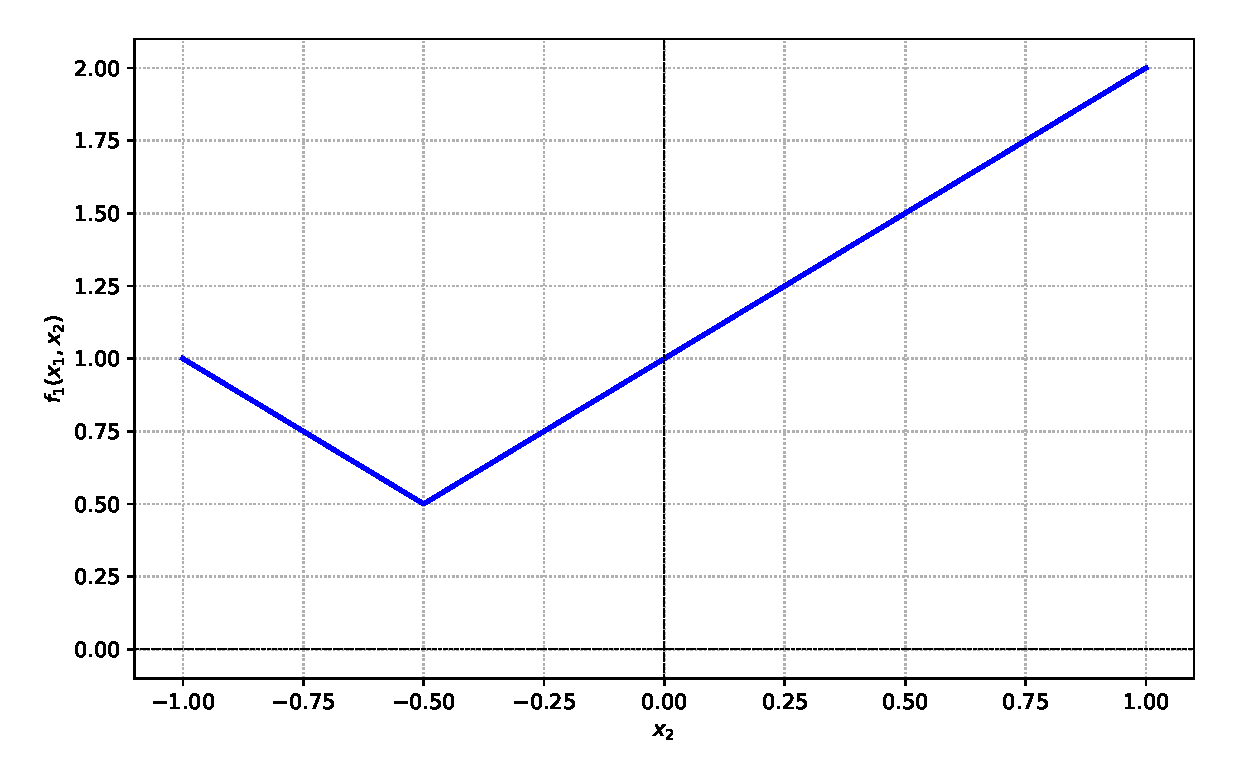
\includegraphics[width=1\textwidth]{graphics/ex3.eps}
	\end{figure}
	\end{frame}
	
\end{comment}
	
	\begin{frame}{Функция, заданная на симплексах}
		Рассмотрим некоторое разбиение области \(\Omega\) на симплексы, пересекающиеся только по граничным точкам. Идея состоит в том, что, задав функцию лишь на всех вершинов данных симплексов, мы сможем продолжить ее на всю область.
	Для каждого симплекса \(\Omega^{(k)}\) обозначим координаты его вершин как \(g^{(k)}_1,\dots,g^{(k)}_n\). Тогда для любой точки \(x \in \Omega^{(k)}\) будет существовать единственный вектор барицентрических координат \(\alpha^{(k)} = \alpha^{(k)}(x) = (\alpha^{(k)}_1,\,\dots, \alpha^{(k)}_{n+1})\) такой, что
	\[\sum_{i = 1}^{n + 1} \alpha^{(k)}_i = 1,\quad \alpha^{(k)}_i \ge 0\ \forall i = \overline{1, n+1},\quad \sum_{i = 1}^{n+1} \alpha^{(k)}_i g^{(k)}_i = x.\]
	\end{frame}
	
	\begin{frame}{Функция, заданная на симплексах}
		Дополним вектор \(x\) до  \(\tilde{x} = \begin{bmatrix} x \\ 1 \end{bmatrix}\), и пусть \(\tilde{G}^{(k)} = \begin{bmatrix} g^{(k)}_{1} & \dots & g^{(k)}_{n+1} \\ 1 & \dots & 1 \end{bmatrix} \in \mathbb{R}^{(n + 1) \times (n + 1)}\). Тогда \(\tilde{G}^{(k)} \alpha^{(k)}(x) = \tilde x\). Пусть \((\tilde{G}^{(k)})^{-1} = \begin{bmatrix} H^{(k)} & h^{(k)} \end{bmatrix}\). Получим, что \(\alpha^{(k)}(x) = H^{(k)} x + h^{(k)} \).
		
		При \(x \in \Omega^{(k)}\) справедливо следующее представление функции \(f\):
		\[f(x) = F^{(k)}\alpha^{(k)}(x) = A^{(k)}x + b^{(k)},\]
		где \[F^{(k)} = \begin{bmatrix} f(g^{(k)}_{1}) & \dots & f(g^{(k)}_{n+1}) \end{bmatrix} \in \mathbb{R}^{n\times(n+1)},\]
		\[A^{(k)} = F^{(k)}H^{(k)} \in \mathbb{R}^{n\times n},\quad b^{(k)} = F^{(k)}h^{(k)} \in \mathbb{R}^{n}.\]
		Таким образом, мы получили явный кусочно-аффинный вид функции на всей области определения и можем применить условие (\ref{qmpwaff}).
	\end{frame}
	\begin{frame}{Общий случай}
		Нахождение кусочно-аффинного вида функции эквивалентно решению системы
		\[
		\begin{cases}
			\sum_{k = 1}^{n}g_{jk}a_{ik} + b_i = f_i(g_j),\ j = \overline{1, n+1}
		\end{cases}
		\]
		относительно \(a_{ik}\) и \(b_i\) для всех \(i = \overline{1, n}\). В дальнейшем будем рассматривать одну систему для некоторого фиксированного \(i\). Можно заметить, что элементы \(a_{ii}\) и \(b_i\) не нужны для проверки, поэтому можно исключить их из системы для упрощения.
	\end{frame}

	\begin{frame}{Случай стандартного разбиения}
		Рассмотрим единичный гиперкуб
		\[
		P = \{x \in \mathbb R^n: 0 \le x_i \le 1, i = \overline{1, n}\}.
		\] 
		Каждый симплекс в разбиении данного \(n\)-мерного куба задается следующим образом: для некоторой перестановки \(\sigma = (\sigma_1, \dots, \sigma_n)\) чисел \(1,\dots,n\)
		\[P_\sigma = \{x \in \mathbb R^n: 0 \le x_{\sigma_1} \le x_{\sigma_2} \le \dots \le x_{\sigma_n} \le 1\}.\]
		Эти симплексы пересекаются лишь по границам и в объединении образуют весь \(n\)-мерный куб. Множество вершин таких симплексов имеет вид
		\[
		\{g_1 = (0,\dots,0), g_2 = e_{\sigma_1}, g_3 = e_{\sigma_1} + e_{\sigma_2}, \dots, g_{n+1} = (1,\dots,1)\},
		\]
		где \(e_j,\ j = \overline{1, n}\) --- единичные векторы.
	\end{frame}
	
	\begin{frame}{Случай стандартного разбиения}
		\begin{figure}[H]
			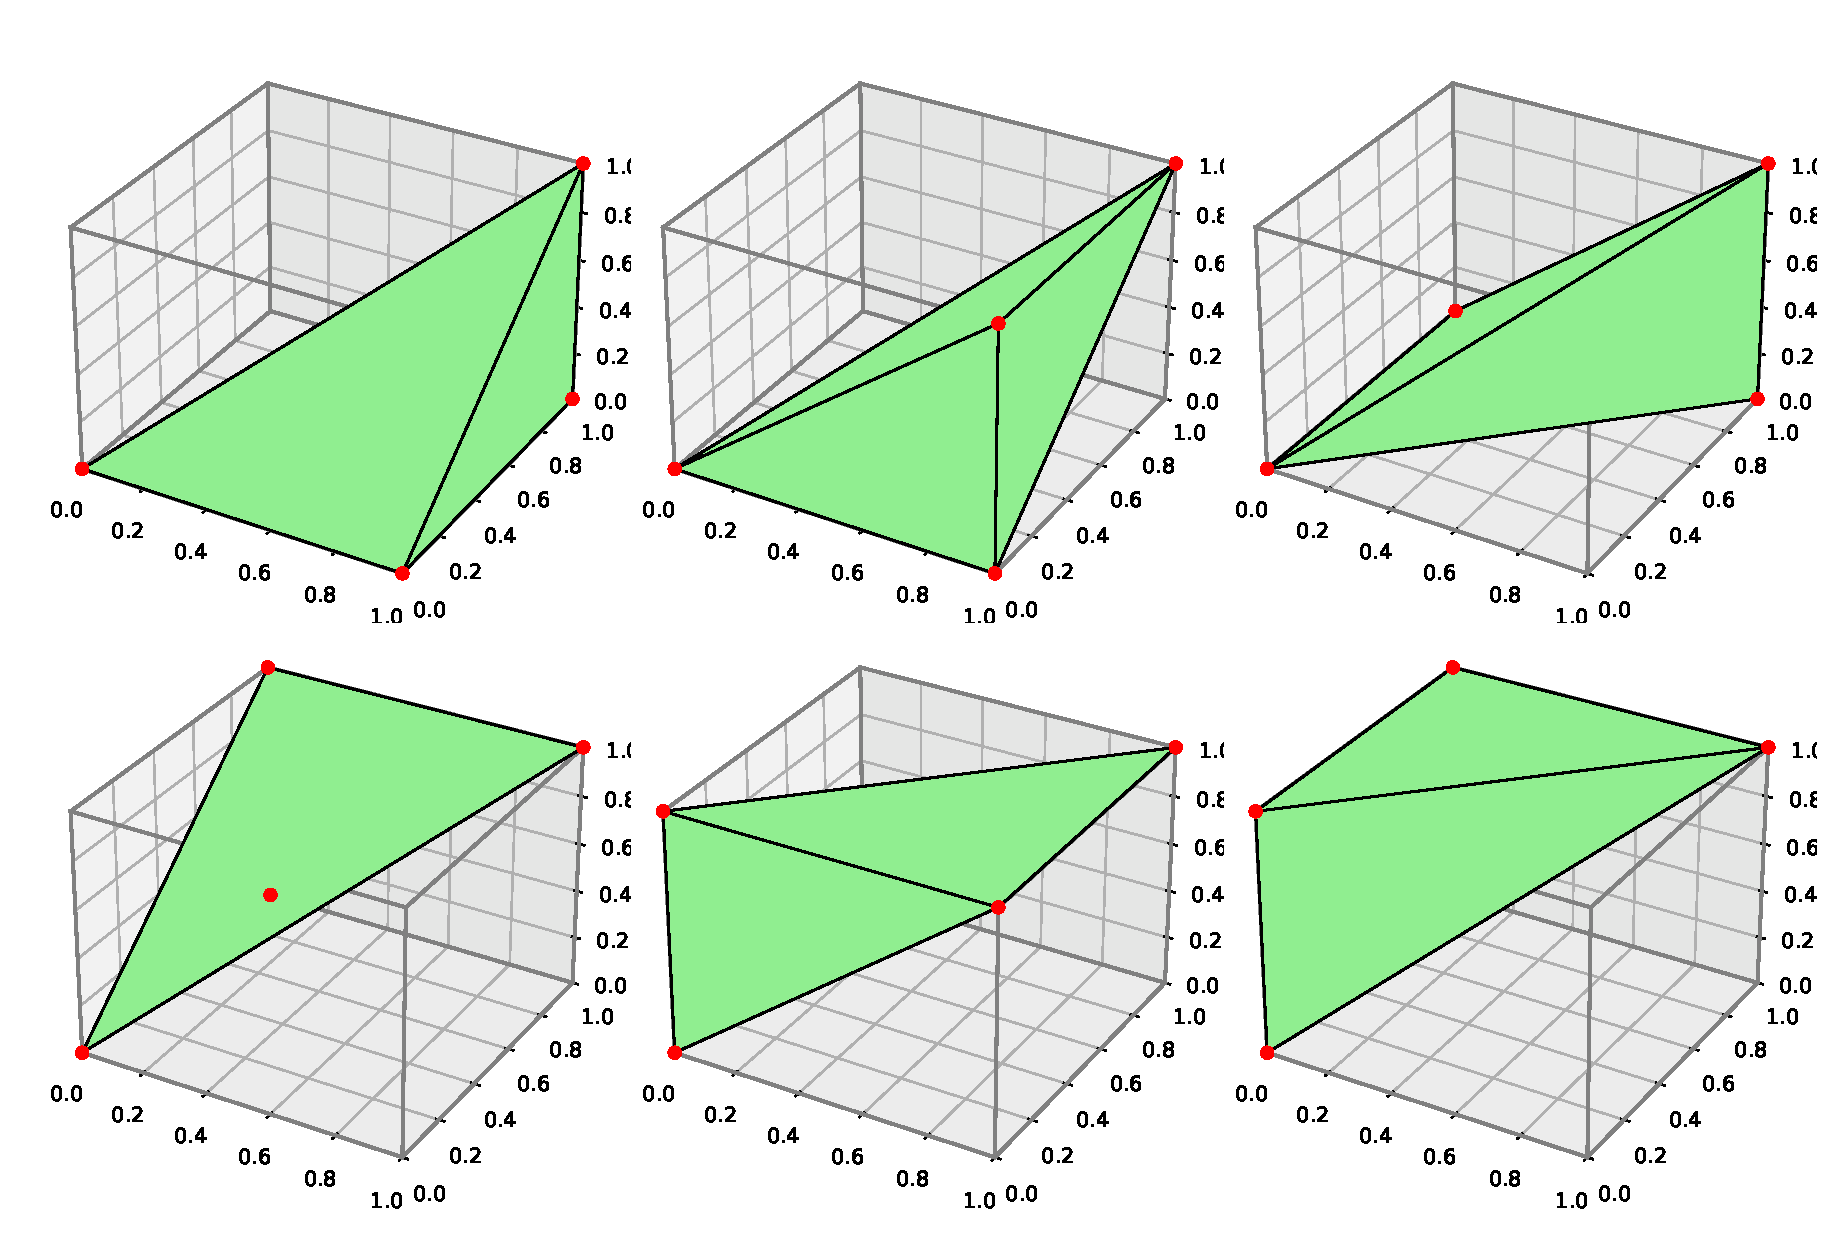
\includegraphics[width=1\textwidth]{graphics/ex2.eps}
			\caption{Стандартное разбиение в трехмерном пространстве}
		\end{figure}
	\end{frame}
	
	\begin{frame}{Критерий для стандартного разбиения}
		Кусочно-аффинная функция, заданная на стандартном разбиении, будет квазимонотонной тогда и только тогда, когда для всех соседних вершин
		\[\alpha = (\alpha_1, \dots, \alpha_{j-1}, \alpha_j, \alpha_{j+1},\dots, \alpha_n),\] \[\beta = (\alpha_1, \dots, \alpha_{j-1}, \alpha_j + 1, \alpha_{j+1},\dots, \alpha_n),\]
		\[i = \overline{1, n},\ j = \overline{1, n},\ j\neq i,\ \alpha_j \in \mathbb Z\]
		таких, что \(\alpha, \beta\) находятся в области определения функции, выполнено
		\[f_i(\beta) \ge f_i(\alpha).\]
	\end{frame}
	
	\begin{frame}{Обобщенная квазимонотонность}
		\begin{rutheorem}
			Рассмотрим систему
			\begin{equation}
				\dot x = f(t, x),\ t\in [t_0,t_1],\ x \in \Omega \subset \mathbb{R}^n,
			\end{equation}
			Функция \(f(t, x)\) непрерывна по \(t\), удовлетворяет условию Липшица по \(x \in \Omega\). Зафиксируем два вектора \(y', y'' \in \Omega\), для которых
			\[\sigma_i y_i' \le \sigma_i y_i''\ \forall i = \overline{1, n},\ \exists j: \sigma_jy_j' < \sigma_j y_j'',\]	
			для некоторых фиксированных чисел \(\sigma_i \in \{-1, 1\},\ i = \overline{1, n}\). 
			
		\end{rutheorem}
	\end{frame}
	
	\begin{frame}{Обобщенная квазимонотонность}
		\begin{rutheorem}
			Пусть функция \(f(t, x)\) удовлетворяет условию квазимонотонности по внедиагональным элементам следующего вида: 
			\begin{multline}
				\sigma_i f_i(t, x_1 + \sigma_1 \alpha_1,\dots, x_{i - 1} + \sigma_{i-1} \alpha_{i-1}, x_i,\\ x_{i+1} + \sigma_{i+1} \alpha_{i+1}, \dots, x_n + \sigma_n \alpha_n) \ge \sigma_i f_i(t, x_1,\dots,x_n)
				\\ \forall t \in [t_0, t_1], x = (x_1,\dots,x_n) \in \Omega,\\ \alpha = (\alpha_1,\dots,\alpha_n) \in \mathbb{R}^n_+,\ i = \overline{1, n}.
			\end{multline}
		\end{rutheorem}
	\end{frame}
	
	\begin{frame}{Обобщенная квазимонотонность}
		\begin{rutheorem}
			Пусть \(x'(t),\ t \in [t_0, t_1]\) --- решение задачи Коши
			\begin{equation}
				\begin{cases} \label{zk1}
					\dot x' = f(t, x'), \\
					x'(t_0) = y'. \\
				\end{cases}
			\end{equation}
			Аналогично определено решение \(x''(t),\ t \in [t_0, t_1]\) задачи Коши
			\begin{equation}
				\begin{cases} \label{zk2}
					\dot x'' = f(t, x''), \\
					x''(t_0) = y''. \\
				\end{cases}
			\end{equation}
			Тогда \(\forall t \in [t_0,t_1]\) справедливы следующие неравенства:
			\begin{equation}
				\sigma_i x_i'(t) \le \sigma_i x_i''(t)\ \forall i = \overline{1,n}.
			\end{equation}
		\end{rutheorem}
	\end{frame}
\end{document}